\documentclass[a4paper,11pt]{article}
\pagestyle{headings}
\usepackage[utf8]{inputenc}
\usepackage[T1]{fontenc}
\usepackage[polish]{babel}
\usepackage{graphicx}
\usepackage{hyperref}
\renewcommand{\familydefault}{\rmdefault}
\renewcommand*\rmdefault{ptm}
\renewcommand*\sfdefault{phv}
\renewcommand*\ttdefault{pcr}
\author{Phitherek\_ SO9PH}
\title{HAM Radio Cheat Sheet}
\begin{document}
\maketitle
\tableofcontents
\section{Krótki wstęp}
W tym dokumencie przedstawiam w skrócie wszelkie informacje potrzebne do przeprowadzenia zgodnie z zasadami łączności radiowej na pasmach amatorskich. Aby samodzielnie przeprowadzić łączność na tych pasmach należy posiadać pozwolenie radiowe. Istnieją kluby krótkofalarskie, w których można taką łączność przeprowadzić pod nadzorem operatora odpowiedzialnego.
\section{Pasma i bandplan}
W zakresie fal krótkich (KF, ang. HF (High Frequency)) oraz ultrakrótkich (UKF, ang. VHF (Very High Frequency, 2m) i UHF (Ultra High Frequency, 70 cm)) istnieją poszczególne pasma, które mają różne właściwości. W każdym paśmie istnieją wydzielone częstotliwości tworzące pasma amatorskie - tylko na tych pasmach można prowadzić amatorską łączność krótkofalarską\footnote{Pasma amatorskie występują także poza wymienionym tu zakresem fal, ale nie są aż tak popularne. Łączności amatorskie bez pozwolenia można prowadzić także w pasmach CB i PMR.}. W ramach tych częstotliwości ustalane są podzakresy i ich przeznaczenie - nazywamy to bandplanem. Bandplan nie jest formalnie wiążący - jest tylko zaleceniem - natomiast w praktyce wszyscy go przestrzegają. Ważniejsze części bandplanu przedstawiam w poniższej tabeli.
\begin{center}
\begin{tabular}{| c | c | p{8cm} |}
\hline
\textbf{Pasmo} & \textbf{Zakres częstotliwości} & \textbf{Przeznaczenie} \\ \hline
80 m & 3500-3580 kHz & CW i dane (szerokość pasma < 200 Hz) \\ \cline{2-3}
 & 3580-3600 kHz & CW, RTTY i dane (szerokość pasma < 500 Hz) \\ \cline{2-3}
 & 3600-3620 kHz & CW, RTTY, dane, transmisje testowe, głos i obraz \\ \cline{2-3}
 & 3620-3800 kHz & CW, głos i obraz (szerokość pasma < 3 kHz) \\ \hline
40 m & 7000-7040 kHz & CW i dane (szerokość pasma < 200 Hz) \\ \cline{2-3}
 & 7040-7050 kHz & CW, RTTY i dane (szerokość pasma < 500 Hz) \\ \cline{2-3}
 & 7050-7060 kHz & CW, RTTY, dane, transmisje testowe, głos i obraz \\ \cline{2-3}
 & 7060-7100 kHz & CW, głos i obraz (szerokość pasma < 3 kHz) \\ \cline{2-3}
 & 7100-7200 kHz & CW, głos i obraz (szerokość pasma < 3 kHz, od marca 2009) \\ \cline{2-3}
 & 7200-7300 kHz & CW, głos i obraz (szerokość pasma < 3 kHz, jako drugorzędne) \\ \hline
30 m & 10100-10140 kHz & CW i dane (szerokość pasma < 200 Hz) \\ \cline{2-3}
 & 10140-10150 kHz & CW, RTTY i dane (szerokość pasma < 500 Hz) \\ \hline
20 m & 14000-14070 kHz & CW i dane (szerokość pasma < 200 Hz) \\ \cline{2-3}
 & 14070-14099 kHz & CW, RTTY i dane (szerokość pasma < 500 Hz) \\ \cline{2-3}
 & 14100 kHz & Zarezerwowane dla beaconów \\ \cline{2-3}
 & 14101-14350 kHz & CW, głos i obraz (szerokość pasma < 3 kHz) \\ \hline
17 m & 18068-18095 kHz & CW i dane (szerokość pasma < 200 Hz) \\ \cline{2-3}
 & 18095-18109 kHz & CW, RTTY i dane (szerokość pasma < 500 Hz) \\ \cline{2-3}
 & 18110 kHz & Zarezerwowane dla beaconów \\ \cline{2-3}
 & 18111-18168 kHz & CW, głos i obraz (szerokość pasma < 3 kHz) \\ \hline
15 m & 21000-21070 kHz & CW i dane (szerokość pasma < 200 Hz) \\ \cline{2-3}
 & 21070-21110 kHz & CW, RTTY i dane (szerokość pasma < 500 Hz) \\ \cline{2-3}
 & 21110-21120 kHz & CW, RTTY, dane, BEZ SSB (szerokość pasma < 2.7 kHz) \\ \cline{2-3}
 & 21120-21149 kHz & CW, RTTY i dane (szerokość pasma < 500 Hz) \\ \cline{2-3}
 & 21150 kHz & Zarezerwowane dla beaconów \\ \cline{2-3}
 & 21151-21450 kHz & CW, RTTY, dane, transmisje testowe, głos i obraz \\ \hline
12 m & 24890-24915 kHz & CW i dane (szerokość pasma < 200 Hz) \\ \cline{2-3}
 & 24915-24929 kHz & CW, RTTY i dane (szerokość pasma < 500 Hz) \\ \cline{2-3}
 & 24930 kHz & Zarezerwowane dla beaconów \\ \cline{2-3}
 & 24931-24990 kHz & CW, głos i obraz (szerokość pasma < 3 kHz) \\ \hline
10 m & 28000-28070 kHz & CW i dane (szerokość pasma < 200 Hz) \\ \cline{2-3}
 & 28070-28190 kHz & CW, RTTY i dane (szerokość pasma < 500 Hz) \\ \cline{2-3}
 & 28191-28224 kHz & Zarezerwowane dla beaconów \\ \cline{2-3}
 & 28225-29200 kHz & CW, głos i obraz (szerokość pasma < 3 kHz) \\ \cline{2-3}
 & 29200-29300 kHz & CW, dane, pakiety, transmisja FM, głos i obraz (szerokość pasma < 20 kHz) \\ \cline{2-3}
 & 29300-29510 kHz & Zarezerwowane na link satelitarny \\ \cline{2-3}
 & 29510-29700 kHz & CW, głos i obraz (szerokość pasma < 3 kHz) \\ \hline
\end{tabular}
\end{center}
\begin{center}
\begin{tabular}{| c | c | p{8cm} |}
\hline
6 m & 50.000-50.100 MHz & CW \\ \cline{2-3}
 & 50.100-50.500 MHz & CW, dane, RTTY, głos i obraz \\ \cline{2-3}
 & 50.500-52.000 MHz & CW, dane, RTTY i głos \\ \hline
2 m & 144.000-144.150 MHz & CW \\ \cline{2-3}
 & 144.150-144.500 MHz & CW i głos \\ \cline{2-3}
 & 144.500-145.000 MHz & CW, dane, RTTY, głos i obraz \\ \cline{2-3}
 & 145.000-146.000 MHz & CW, dane, RTTY, głos i obraz \\ \hline
70 cm & 430.000-432.000 MHz & CW, dane, RTTY, głos, obraz i TV \\ \cline{2-3}
 & 432.000-432.100 MHz & CW \\ \cline{2-3}
 & 432.100-432.400 MHz & CW, głos \\ \cline{2-3}
 & 432.400-440.000 MHz & CW, dane, RTTY, dane pakietowe, głos, obraz i TV \\ \hline
\end{tabular}
\end{center}
\subsection{Krótko o typach emisji}
\begin{itemize}
\item Emisja CW - to po prostu telegrafia, czyli porozumiewanie się poprzez nadawanie kodu Morse' a. Polega na przerywaniu niemodulowanej fali nośnej czyli kluczowaniu.
\item Emisja RTTY - to dalekopis.
\item Dane - to jakakolwiek transmisja cyfrowa.
\item Pakiety - transmisja PacketRadio.
\item Głos - inaczej transmisja foniczna, wykorzystuje głos ludzki. Istnieją trzy jej główne typy - FM, AM i wstęgowa (SSB), która dzieli się na dolnowstęgową (LSB) i górnowstęgową (USB).
\item Obraz - transmisja obrazu przez SSTV.
\end{itemize}
\subsection{Uwagi do bandplanu UKF}
Poniżej zamieszczam szczegółowe zastosowania zakresów częstotliwości w pasmach UKF.
\begin{center}
\begin{tabular}{| c | c | p{8cm} |}
\hline
\textbf{Pasmo} & \textbf{Zakres częstotliwości} & \textbf{Przeznaczenie} \\ \hline
2 m & 144.150-144.399 MHz & SSB \\ \cline{2-3}
 & 144.400-144.491 MHz & Radiolatarnie \\ \cline{2-3}
 & 145.000-145.194 MHz & Wejścia przemienników amatorskich \\ \cline{2-3}
 & 145.206-145.594 MHz & Simplex transmisji FM \\ \cline{2-3}
 & 145.600-145.794 MHz & Wyjścia przemienników amatorskich \\ \cline{2-3}
 & 145.800-146.000 MHz & Pasmo łączności satelitarnej \\ \hline
70 cm & 431.050-431.825 MHz & Wejścia przemienników amatorskich \\ \cline{2-3}
 & 432.400-432.490 MHz & Radiolatarnie \\ \cline{2-3}
 & 435.000-438.000 MHz & Pasmo łączności satelitarnej \\ \cline{2-3}
 & 438.650-439.425 MHz & Wyjścia przemienników amatorskich \\ \hline
\end{tabular}
\end{center}
\section{Znaki, literowanie i łamanie}
W tej części opisuję w jaki sposób identyfikować się w łączności amatorskiej.
\subsection{Znaki krótkofalarskie}
Krótkofalarski znak wywoławczy złożony jest z dwóch znaków alfanumerycznych (liter lub cyfr) zwanych prefiksem, następnie numerem, a następnie kolejnymi znakami alfanumerycznymi zwanymi sufiksem, których ilość jest zależna od przepisów danego kraju. W Polsce długość sufiksu ma od 1 do 4 znaków (stacje okolicznościowe do 7 znaków). Przykłady znaków to SQ9O, SO9PH, SQ9WTF lub SP9HACK. Znak krótkofalarski służy do jednoznacznej identyfikacji nadającej stacji.
\subsection{Literowanie}
Aby nasz znak oraz inne przekazywane informacje były zrozumiałe dla odbiorcy, zwłaszcza przy dużych zakłóceniach, stosuje się literowanie. Istnieją literowania specyficzne dla języków oraz literowanie międzynarodowe ITU. W poniższej tabeli przedstawiam najczęściej stosowane literowania - polskie, międzynarodowe i angielskie.
\begin{center}
\begin{tabular}{| c | p{4cm} | p{4cm} | p{4cm} |}
\hline
\textbf{Litera} & \textbf{Literowanie polskie} & \textbf{Literowanie ITU (NATO)} & \textbf{Literowanie angielskie} \\ \hline
A & Adam & Alpha (czyt. alfa) & Able (czyt. ejbl) \\ \hline
B & Barbara & Bravo (czyt. brawo) & Baker (czyt. bejker) \\ \hline
C & Celina/Cezary & Charlie (czyt. czarli) & Charlie (czyt. czarli) \\ \hline
D & Dorota & Delta (czyt. delta) & Dog (czyt. dog) \\ \hline
E & Ewa & Echo (czyt. ekou) & Easy (czyt. izi) \\ \hline
F & Franciszek/Franek & Foxtrot (czyt. fokstrot) & Fox (czyt. foks) \\ \hline
G & Genowefa/Grażyna & Golf (czyt. golf) & George (czyt. dżordż) \\ \hline
H & Henryk/Halina & Hotel (czyt. hotel) & How (czyt. hau) \\ \hline
I & Irena & India (czyt. india) & Item (czyt. ajtem) \\ \hline
J & Jadwiga/Józef & Juliett (czyt. dżuliet) & Jig (czyt. dżig) \\ \hline
K & Karol & Kilo (czyt. kilo) & King (czyt. king) \\ \hline
L & Ludwik & Lima (czyt. lima) & Love (czyt. low) \\ \hline
M & Maria & Mike (czyt. majk) & Mike (czyt. majk)/Mary (czyt. mery) \\ \hline
N & Natalia & November (czyt. nowember) & Nan (czyt. nan) \\ \hline
O & Olga & Oscar (czyt. oskar) & Oboe (czyt. oboi) \\ \hline
P & Paweł & Papa (czyt. papa) & Peter (czyt. piter) \\ \hline
Q & Quebec (czyt. kłebek/kebek)/Quantum (czyt. kłantum, rzadziej) & Quebek (czyt. kłebek/kebek) & Queen (czyt. kłin) \\ \hline
R & Roman & Romeo (czyt. romio) & Roger (czyt. rodżer) \\ \hline
S & Stefan & Sierra (czyt. siera) & Sugar (czyt. szuger) \\ \hline
T & Tadeusz & Tango (czyt. tango) & Tare (czyt. tejr) \\ \hline
U & Urszula & Uniform (czyt. juniform) & Uncle (czyt. ankl) \\ \hline
V & Violetta (czyt. wjoletta) & Victor (czyt. wiktor) & Victor (czyt. wiktor) \\ \hline
W & Wanda & Whiskey (czyt. łiski) & William (czyt. łiliam) \\ \hline
X & Xawery (czyt. ksawery)/Ksantypa (rzadziej) & X-ray (czyt. eks-rej) & X-ray (czyt. eks-rej) \\ \hline
Y & Yokohama (czyt. jokohama)/Ypsylon & Yankee (czyt. janki) & Yoke (czyt. jołk) \\ \hline
Z & Zygmunt & Zulu (czyt. zulu) & Zebra (czyt. zibra) \\ \hline
\end{tabular}
\end{center}
\begin{center}
\begin{tabular}{| c | p{4cm} | p{4cm} |}
\hline
\textbf{Cyfra/Znak} & \textbf{Literowanie polskie} & \textbf{Literowanie ITU (NATO)} \\ \hline
0 & Zero & Zero (czyt. ziro)/Nadazero (czyt. nadazejro) \\ \hline
1 & Jedynka & One (czyt. łan/łun)/Unaone (czyt. unałan/unałun) \\ \hline
2 & Dwa & Two (czyt. tu)/Bissotwo (czyt. bissotu) \\ \hline
3 & Trzy & Three (czyt. tri)/Terrathree (czyt. tejratri) \\ \hline
4 & Cztery & Four (czyt. fołer)/Kartefour (czyt. kartejfołer) \\ \hline
5 & Piątka & Five (czyt. fajf(i))/Pantafive (czyt. pantafajf) \\ \hline
6 & Sześć & Six (czyt. siks)/Soxisix (czyt. soksisiks) \\ \hline
7 & Siedem & Seven (czyt. sewen)/Setteseven (czyt. sejtejsewen) \\ \hline
8 & Osiem & Eight (czyt. ejt)/Oktoeight (czyt. oktoejt) \\ \hline
9 & Dziewięć & Nine (czyt. najn)/Niner (czyt. najner)/Novenine (czyt. nowejnajner) \\ \hline
100 & Sto & Hundred (czyt. handred) \\ \hline
1000 & Tysiąc & Thousand (czyt. tołzand) \\ \hline
Punkt dziesiętny & Punkt dziesiętny & Point/Decimal (czyt. dejsimal) \\ \hline
. & Kropka & Stop (czyt. stop) \\ \hline
\end{tabular}
\end{center}
\subsection{Łamanie}
Łamanie znaku pozwala w prosty sposób przekazać już przy wywołaniu pewne informacje, które mogą być istotne dla pomyślnego przeprowadzenia łączności lub oceny jej atrakcyjności (np. czy łączność jest daleka, czy bliska). Poniżej przedstawiłem najczęściej używane sposoby łamania znaku:
\begin{itemize}
\item ZN4K/p - zwykle literowane ''przez Paweł'', ''przez portable'', po angielsku ''stroke portable'', oznacza że nadajemy ze stacji przenośnej, ręcznej, zwykle małej mocy (QRP).
\item ZN4K/m - zwykle literowane ''przez mobil'', po angielsku ''stroke mobile'' - stacja poruszająca się, najczęściej samochodowa, ale może być też stosowane np. na jachcie żaglowym na wodach terytorialnych.
\item ZN4K/mm - zwykle literowane po angielsku ''Mary Mary'' lub ''Mickey Mouse'' - oznacza stację nadającą ze statku znajdującego się na wodach międzynarodowych.
\item ZN4K/am - nie spotkałem się ze specjalnym literowaniem - oznacza stację pracującą z powietrza.
\item ZN4K/d - po angielsku ''stroke disaster'' - oznacza stację pracującą z miejsca katastrofy lub klęski żywiołowej.
\item PX/ZN4K - jeżeli jesteśmy na terenie innego kraju i jest on w zrzeszeniu CEPT (w przypadku pozwoleń wydanych w krajach tego zrzeszenia, w tym w Polsce), to przez okres 3 miesięcy możemy korzystać ze swojego znaku łamiąc go na początku przez prefiks danego kraju np. OK/ZN4K jeżeli pracujemy z terenu Czech. To jedyne łamanie, które jest obowiązkowe.
\item ZN4K/numer - używane, jeżeli stacja nie łamie się przez nic, a pracuje spoza swojej lokalizacji widniejącej na pozwoleniu radiowym, w szczególności z innego okręgu wywoławczego.
\item QRP - nie jest to typowe łamanie znaku, ale w ten sposób przekazywana jest informacja, że stacja jest małej mocy. Przykłady: \textit{This is QRP station SO9PH} lub \textit{SO9PH QRP}.
\end{itemize}
Opisane powyżej łamania znaków można ze sobą łączyć, aby przekazać dodatkowe informacje. Oczywiście można się też łamać przez inne rzeczy zależnie od sytuacji, ale występują one rzadko. Poniżej przedstawiam mapę polskich okręgów wywoławczych jako załącznik do przedostatniego przykładu.
\begin{figure}[p]
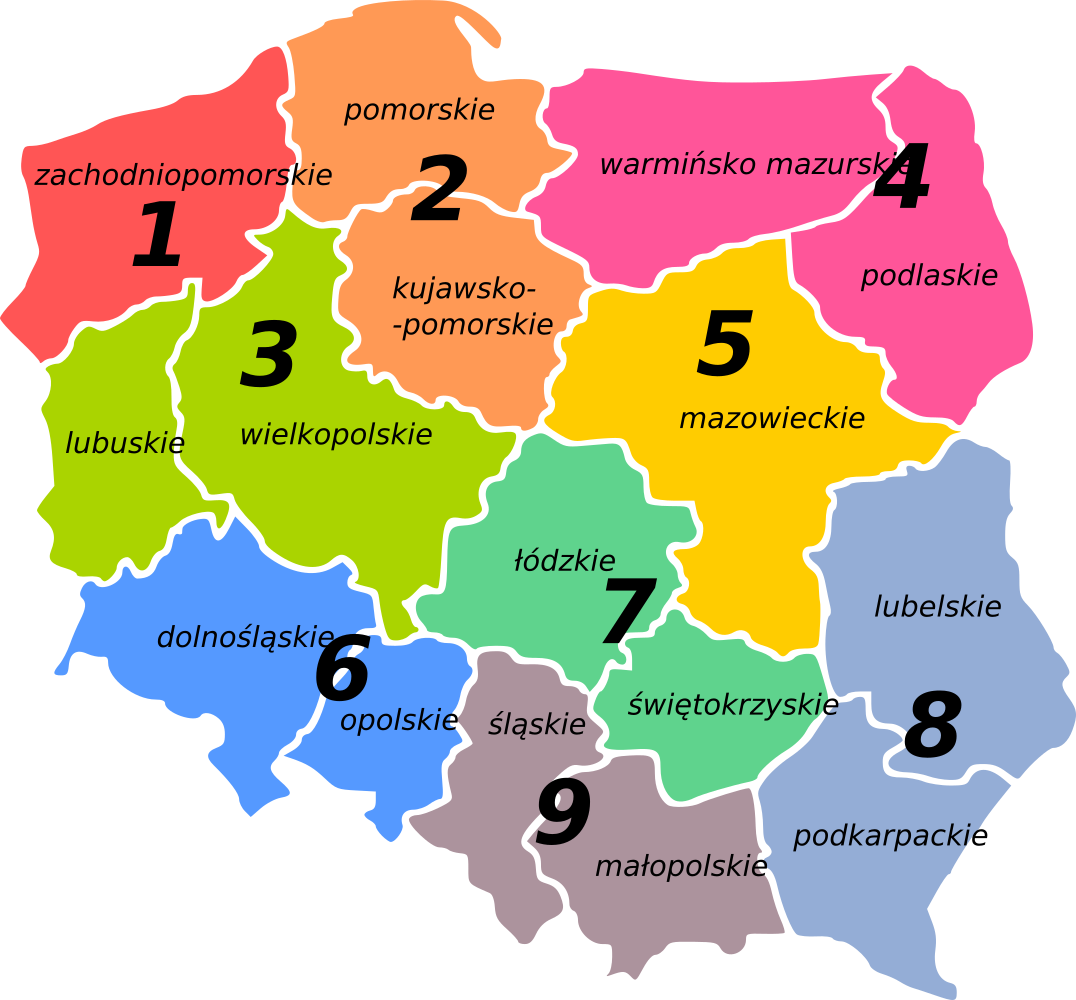
\includegraphics{Polish_HAM_Radio_Regions}
\caption{Polskie okręgi wywoławcze}
\end{figure}
\clearpage
\section{Kod Q i slang radioamatorski}
Kod Q i slang radioamatorski zostały stworzone głównie na potrzeby telegrafii, ale niektórych zwrotów używa się także w łączności głosowej. Służą skróceniu przekazywanej informacji. Najczęściej używane zwroty przedstawiłem w poniższej tabeli.
\begin{center}
\begin{tabular}{| c | c |}
\hline
\textbf{Zwrot} & \textbf{Znaczenie} \\ \hline
QSY & Przejście na częstotliwość, zmiana częstotliwości \\ \hline
QRM & Zakłócenia od innych stacji \\ \hline
QRN & Zakłócenia atmosferyczne (zwłaszcza: burza) \\ \hline
QRV & Gotowość do pracy, bycie czynnym w eterze \\ \hline
QRT & Wyłączam radio, zaprzestaję pracy \\ \hline
QTH & Lokalizacja, położenie geograficzne \\ \hline
QRO & Duża moc, także: zwiększ moc, zwiększam moc \\ \hline
QRP & Mała moc, także: zmniejsz moc, zmniejszam moc \\ \hline
QSO & Łączność \\ \hline
QSL & Potwierdzenie łączności, także karta potwierdzająca łączność \\ \hline
QRZ & Kto mnie wołał? Używane także zamiast wywołania ogólnego. \\ \hline
CQ & Wywołanie ogólne (może być bardziej szczegółowe np. CQ CONTEST) \\ \hline
UNLIS & Nielicencjonowany nadawca \\ \hline
YL & Panna, młoda pani \\ \hline
XYL & Narzeczona, żona, dziewczyna \\ \hline
DX & Daleka łączność \\ \hline
UTC & Czas uniwersalny \\ \hline
LOG & Dziennik pracy stacji \\ \hline
DIRECT & Łączność bezpośrednia \\ \hline
73! & Pozdrowienia amatorskie \\ \hline
99! & Idź precz, przepadnij \\ \hline
\end{tabular}
\end{center}
\section{Przebieg łączności}
W tej sekcji podam podstawowe zasady prowadzenia łączności krótkofalarskiej i przedstawię jak wygląda przykładowa łączność.
\subsection{Podstawowe elementy wymagane w łączności}
W teorii wszystkie wiadomości nadawane w łączności powinny być adresowane do innej stacji, a w wiadomości powinien pojawić się znak zarówno odbiorcy, jak i własny. W praktyce to zależy od sytuacji, ale podawane w łączności znaków jest zawsze mile widziane. Znaki powinno się podawać obok siebie, zaczynając od znaku odbiorcy, a następnie podając własny znak. Aby ułatwić sprawę, warto między te znaki włożyć frazę ''tu'', ''tutaj'' czy ''tutaj stacja''. Przykład: \textit{SO9PH, tutaj SP9HACK}. Aby łączność była formalnie ważna, obie stacje muszą ze sobą wymienić raporty RST, imiona operatorów i lokalizacje (QTH). Znaki warto literować, zwłaszcza na początku łączności, kiedy obie strony muszą je poznać.
\subsection{Wywołanie}
Łączność krótkofalarska zazwyczaj zaczyna się od wywołania. Wywołanie może być ogólne lub bardziej szczegółowe - od programów dyplomowych typu SOTA, poprzez wołanie tylko łączności z dalekich krajów (tzw. DX-ów) czy zawody, po wołanie konkretnego znaku. W wywołaniu ogólnym powinno się też podawać pasmo, ale tylko jeżeli chodzi o wołanie na częstotliwościach bezpośrednich (tzw. DIRECT). Na tych częstotliwościach wywołanie powinno być też dłuższe, aby osoba po drugiej stronie zrozumiała nas przez ewentualne zakłócenia. Przykładowe wywołania:
\begin{itemize}
\item Wywołanie ogólne na częstotliwości bezpośredniej: \textit{Wywołanie ogólne, wywołanie ogólne w paśmie dwóch metrów, tutaj stacja SO9PH, zapraszam do łączności.}
\item Wywołanie ogólne na przemienniku\footnote{Przemiennik to automatyczna stacja, która przekazuje sygnał odbierany na częstotliwości wejściowej na częstotliwość wyjściową. Często znajduje się na wzniesieniu, gdyż jego celem jest zwiększenie zasięgu łączności dla stacji, które do niego docierają i go słyszą. Łączność przez przemiennik nazywa się też dupleksem, w odróżnieniu od simpleksu.}: \textit{Wywołanie ogólne, wywołanie ogólne, tutaj stacja SO9PH, zapraszam do łączności.}
\item Wywołanie w programie górskim SOTA: \textit{Wywołanie, wywołanie w programie SOTA, wywołanie w programie SOTA, tutaj stacja SO9PH, zapraszam do łączności}
\item Wywołanie szczegółowego znaku: \textit{SP9HACK, SO9PH prosi.}
\item Wywołanie po angielsku w paśmie 20 m: \textit{CQ, CQ twenty, CQ twenty, this is SO9PH, calling CQ, standing by for call.}
\end{itemize}
\subsection{Zanim zaczniesz wołać}
Przed rozpoczęciem wołania na częstotliwości bezpośredniej, warto spytać parę razy: \textit{Czy częstotliwość jest wolna? Czy częstotliwość jest wolna? Is the frequency in use?} Po każdym takim zawołaniu zostawić chwilkę przerwy - jeżeli częstotliwość nie jest wolna, powinien zgłosić się operator innej stacji i powiedzieć, że prowadzi łączność. Wtedy należy zaczekać. Jeżeli nie ma odpowiedzi, to można spokojnie zacząć wywołanie. Dlaczego to jest potrzebne? Ponieważ nie zawsze słyszymy obie stacje prowadzące ze sobą łączność.
\subsection{Raport RST}
Raport RST (ang. Readability, Signal, Tone) to trzycyfrowy raport, który daje drugiej stacji ważne informacje o sygnale i łączności z jego strony. Trzeba pamiętać, że jak nadajemy to siebie nie słyszymy, a taki raport może nam pomóc zdiagnozować usterkę w instalacji. Tak samo działa to po drugiej stronie. Raport składa się z trzech części:
\begin{itemize}
\item Czytelność (ang. Readability) - oceniana na ucho w skali od 1 do 5 (1 - zupełnie nieczytelny, 5 - doskonale czytelny)
\item Sygnał (ang. Signal) - czytany z S-metru w radiu w skali od 1 do 9
\item Ton (ang. Tone) - oceniany na ucho w skali od 1 do 9
\end{itemize}
W łączności głosowej używa się tylko dwóch pierwszych kryteriów (RS), ponadto na przemiennikach używa się tylko czytelności (można dodatkowo podać raport RS dla samego przemiennika, głównie jeżeli nie słyszymy go na 59). Cyfry raportu podaje się bezpośrednio po sobie, w kolejności Czytelność, Sygnał Ton, na przykład: \textit{Raport dla Ciebie to 59 (pięć dziewięć)./Słyszę Cię na 59.}
\subsection{Przemienniki i prośba o raport}
Przed rozpoczęciem łączności przez przemiennik często warto zapytać o raport: \textit{Poproszę o raport na przemienniku, tutaj SO9PH.} lub \textit{Czy jestem odbierany na przemienniku? Tutaj SO9PH.} Odpowiedź na taką prośbę brzmi na przykład: \textit{Piątka kolego, tu SP9HACK.} Po odpowiedzi warto podziękować i przekazać krótkie pozdrowienia 73.
\subsection{Praca w grupie}
Jeżeli chcemy się włączyć do prowadzonej rozmowy, to najpierw cierpliwie czekamy, aż stacja skończy nadawać i będzie chwilowa przerwa. W tej przerwie nadajemy raz lub parę razy słowo BREK. Dlatego też zawsze warto zostawiać podczas łączności trochę dłuższą przerwę przed rozpoczęciem nadawania, aby zostawić miejsce dla ewentualnych innych osób. Jeżeli od osoby, do której był aktualnie przekazywany mikrofon, usłyszymy \textit{Proszę bardzo BREK} to możemy się przywitać, podać swój znak i przekazać mikrofon dalej. Przekazywanie mikrofonu odbywa się poprzez nadanie np. \textit{Mikrofon do SP9HACK.} albo po prostu \textit{SP9HACK SO9PH}. Będąc w grupie odzywamy się dopiero wtedy, kiedy zostanie do nas przekazany mikrofon. Przy wymianie znaków wymieniamy tylko znak stacji, która nam przekazała i dodajemy: \textit{i grupa} lub \textit{i ewentualna grupa} jeżeli nie wiemy, czy ktoś jeszcze prowadzi wraz z nami rozmowę.
\subsection{Kończenie transmisji}
Aby miło skończyć transmisję, należy podziękować za łączność i przekazać pozdrowienia dla naszego rozmówcy. Nie należy zupełnie kończyć łączności dopóki druga strona nie odpowie nam tym samym. Jeżeli jesteśmy ostatnią stacją w łączności, warto wymienić znaki i ewentualnie imiona i lokalizacje stacji, które uczestniczyły włączności, wyrażnie zaznaczyć koniec łączności i że częstotliwość lub przemiennik są już wolne.
\subsection{Przykładowe łączności}
Chciałbym podsumować powyższe informacje poprzez podanie pełnych przykładowych łączności po polsku i po angielsku. Poniżej przedstawiam przykładową łączność w języku polskim pomiędzy stacjami SO9PH i SP9HACK przez przemiennik:
\begin{itemize}
\item \textit{Wywołanie ogólne, wywołanie ogólne, tutaj stacja Stefan Olga Dziewięć Paweł Halina, zapraszam do łączności.}
\item \textit{Stefan Paweł Dziewięć Halina Adam Cezary Karol}
\item \textit{Stefan Paweł Dziewięć Halina Adam Cezary Karol, tutaj Stefan Olga Dziewięć Paweł Halina. Witam kolegę serdecznie, z tej strony operator Piotr, moje QTH to Kraków, odbieram cię na piątkę, bardzo ładnie. Mikrofon do Ciebie.}
\item \textit{Stefan Olga Dziewięć Paweł Halina, tutaj Stefan Paweł Dziewięć Halina Adam Cezary Karol. Również serdecznie wita, z tej strony operator Paweł, moje QTH to też Kraków. Raport dla Ciebie to także bardzo ładna piątka. Mikrofon do Ciebie.}
\item \textit{SP9HACK tu SO9PH, fajnie było Cię spotkać. Dziękuję Ci za łączność, 73 i do następnych. Mikrofon na finał do Ciebie.}
\item \textit{SO9PH tu SP9HACK, również fajnie Cię słyszeć, dziękuję za miłe krótkie QSO, 73 i do następnych spotkań. Rozmawiały stacje Stefan Olga Dziewięć Paweł Halina (Piotr, Kraków) i Stefan Paweł Dziewięć Halina Adam Cezary Karol (Paweł, Kraków). Po łączności, przemiennik wolny.}
\end{itemize}
A poniżej łączność między tymi samymi stacjami po angielsku na częstotliwości bezpośredniej:
\begin{itemize}
\item \textit{CQ, CQ two meter, CQ two meter this is Sierra Oscar Nine Papa Hotel, calling CQ, standing by for call.}
\item \textit{Sierra Papa Nine Hotel Alpha Charlie Kilo}
\item \textit{Sierra Papa Nine Hotel Alpha Charlie Kilo, this is Sierra Oscar Nine Papa Hotel. Hello, this is operator Piotr, this is Papa India Oscar Tango Romeo, my current QTH is Cracow, this is Charlie Romeo Alpha Charlie Oscar Whiskey. The report for you is five nine. Go ahead.}
\item \textit{Sierra Oscar Nine Papa Hotel, this is Sierra Papa Nine Hotel Alpha Charlie Kilo. Hello Piotr, nice to meet you, this is operator Paweł, this is Papa Alpha Whiskey Echo Lima, my current QTH is also Cracow. The report for you is also five nine. Go ahead.}
\item \textit{Sierra Papa Nine Hotel Alpha Charlie Kilo, this is Sierra Oscar Nine Papa Hotel. Thank you very much for QSO, 73 to you and all the best. Go ahead.}
\item \textit{Sierra Oscar Nine Papa Hotel, this is Sierra Papa Nine Hotel Alpha Charlie Kilo. Also thank you for QSO, 73 and all the best. Sierra Oscar Nine Papa Hotel and Sierra Papa Nine Hotel Alpha Charlie Kilo were talking, QSO over, frequency free.}
\end{itemize}
\section{Log stacji i logowanie łączności}
Łączności warto zapisywać w logu. Log stacji to papierowy lub elektroniczny zapis łączności. Zawiera zwykle znak korespondenta, raporty do i od drugiej strony, imię i QTH rozmówcy oraz datę i godzinę UTC łączności. Można także zapisywać częstotliwość i modulację. Prowadzenie logu jest wskazane, ale nie jest wymagane. Przykładowy wpis do logu:
\begin{center}
\begin{tabular}{| c | c | c | c | c | c |}
\hline
\textbf{Znak} & \textbf{Raport do} & \textbf{Raport od} & \textbf{Imię} & \textbf{QTH} & \textbf{UTC} \\ \hline
SP9HACK & 59 & 59 & Paweł & Kraków & 25.01.2016 10:00 \\ \hline
\end{tabular}
\end{center}
\section{Chcesz wiedzieć więcej?}
W tym dokumencie tylko liznąłem temat krótkofalarstwa, gromadząc mam nadzieję wszystkie informację potrzebne do prawidłowego przeprowadzenia pierwszych łączności. Jeżeli spodobał Ci się, drogi czytelniku, temat i chciałbyś dowiedzieć się więcej lub szukasz już materiałów na egzamin, serdecznie polecam \href{http://kurs.sp9kgp.org}{stronę kursu klubu Ryjek SP9KGP}. Polecam również Google i Wikipedię - zwłaszcza źródła angielskie. To właśnie z tych źródeł powstał niniejszy dokument, wspierany moim własnym doświadczeniem operatorskim. Amatorskie 73, dalekich łączności i owocnego korzystania z powyższych informacji życzy Phitherek\_ SO9PH. Do usłyszenia na pasmach!
\section{Podziękowania}
Chciałbym podziękować za wkład w ulepszenie tego dokumentu następującym osobom:
\begin{itemize}
\item Wojtkowi SQ9PBS za uwagi merytoryczne.
\end{itemize}
\end{document}